
%{{第五回}}{第五回}}

\chapter{开生面梦演红楼梦\hspace{.5em}立新场情传幻境情}
{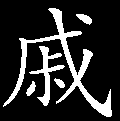
\includegraphics[width=3mm]{../Images/00005}\kaishu 万种豪华原是幻,何尝造孽,何是风流?曲终人散有谁留,为甚营求?只爱蝇头!一番遭遇几多愁,点水根由,泉涌难酬!}

题曰:

春困葳蕤拥绣衾,恍随仙子别红尘。

问谁幻入华胥境?千古风流造孽人。\href{../Text/part0009_split_000.html\#lnkback_1_a}{\textsuperscript{①}}

却说薛家母子在荣府中寄居等事略已表明,此回则暂不能写矣。{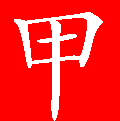
\includegraphics[width=3mm]{../Images/00002}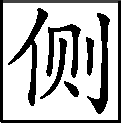
\includegraphics[width=3mm]{../Images/00011}\footnotesize \kaishu 此等处实又非别部小说之熟套起法。}

如今且说林黛玉{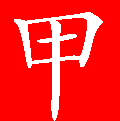
\includegraphics[width=3mm]{../Images/00002}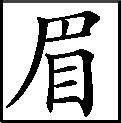
\includegraphics[width=3mm]{../Images/00010}\footnotesize \kaishu 不叙宝钗,反仍叙黛玉。盖前回只不过欲出宝钗,非实写之文耳,此回若仍续写,则将二玉高搁矣,故急转笔仍归至黛玉,使荣府正文方不至于冷落也。◇今写黛玉,神妙之至,何也?因写黛玉实是写宝钗,非真有意去写黛玉,几乎又被作者瞒过。}自在荣府以来,贾母万般怜爱,寝食起居,一如宝玉,{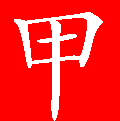
\includegraphics[width=3mm]{../Images/00002}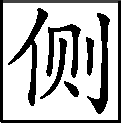
\includegraphics[width=3mm]{../Images/00011}\footnotesize \kaishu 妙极!所谓一击两鸣法,宝玉身份可知。}迎春、探春、惜春三个亲孙女倒且靠后。{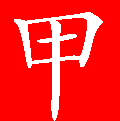
\includegraphics[width=3mm]{../Images/00002}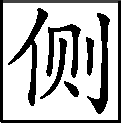
\includegraphics[width=3mm]{../Images/00011}\footnotesize \kaishu 此句写贾母。}便是宝玉和黛玉二人之亲密友爱,亦自较别个不同,{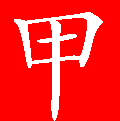
\includegraphics[width=3mm]{../Images/00002}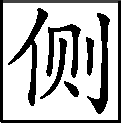
\includegraphics[width=3mm]{../Images/00011}\footnotesize \kaishu 此句妙,细思有多少文章。}日则同行同坐,夜则同息同止,真是言和意顺,略无参商。不想如今忽然来了一个薛宝钗,{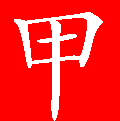
\includegraphics[width=3mm]{../Images/00002}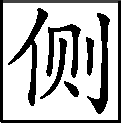
\includegraphics[width=3mm]{../Images/00011}\footnotesize \kaishu 总是奇峻之笔,写来健拔,似新出之一人耳。}年岁虽大不多,然品格端方,容貌丰美,{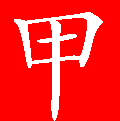
\includegraphics[width=3mm]{../Images/00002}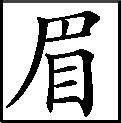
\includegraphics[width=3mm]{../Images/00010}\footnotesize \kaishu 此处如此写宝钗,前回中略不一写,可知前回迥非十二钗之正文也。◇欲出宝钗,便不肯从宝钗身上写来,却先款款叙出二玉,陡然转出宝钗,三人方可鼎立。行文之法又一变体。}人多谓黛玉所不及。{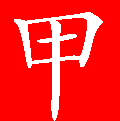
\includegraphics[width=3mm]{../Images/00002}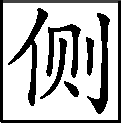
\includegraphics[width=3mm]{../Images/00011}\footnotesize \kaishu 此句定评,想世人目中各有所取也。按黛玉宝钗二人,一如姣花,一如纤柳,各极其妙者,然世人性分甘苦不同之故耳。}而且宝钗行为豁达,随分从时,不比黛玉孤高自许,目无下尘。{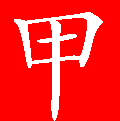
\includegraphics[width=3mm]{../Images/00002}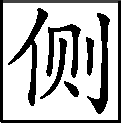
\includegraphics[width=3mm]{../Images/00011}\footnotesize \kaishu 将两个行止摄总一写,实是难写,亦实系千部小说中未敢写者。}故比黛玉大得下人之心。便是那些小丫头子们,亦多喜与宝钗去顽笑。因此黛玉心中便有些悒郁不忿之意,{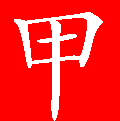
\includegraphics[width=3mm]{../Images/00002}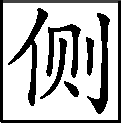
\includegraphics[width=3mm]{../Images/00011}\footnotesize \kaishu 此一句是今古才人同病,如人人皆如我黛玉之为人,方许他妒。◇此是黛玉缺处。}宝钗却浑然不觉。{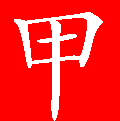
\includegraphics[width=3mm]{../Images/00002}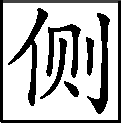
\includegraphics[width=3mm]{../Images/00011}\footnotesize \kaishu 这还是天性,后文中则是又加学力了。}那宝玉亦在孩提之间,况自天性所禀来的一片愚拙偏僻,{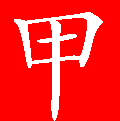
\includegraphics[width=3mm]{../Images/00002}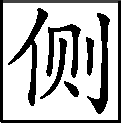
\includegraphics[width=3mm]{../Images/00011}\footnotesize \kaishu 四字是极不好,却是极妙。只不要被作者瞒过。}视姊妹弟兄皆出一体,并无亲疏远近之别。{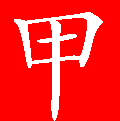
\includegraphics[width=3mm]{../Images/00002}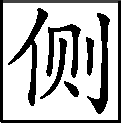
\includegraphics[width=3mm]{../Images/00011}\footnotesize \kaishu 如此反谓``愚痴'',正从世人意中写也。}其中因与黛玉同随贾母一处坐卧,故略比别个姊妹熟惯些。既熟惯,则更觉亲密,既亲密,则不免一时有求全之毁、不虞之隙。{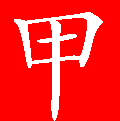
\includegraphics[width=3mm]{../Images/00002}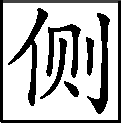
\includegraphics[width=3mm]{../Images/00011}\footnotesize \kaishu 八字定评,有趣。不独黛玉、宝玉二人,亦可为古今天下亲密人当头一喝。 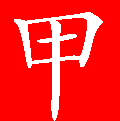
\includegraphics[width=3mm]{../Images/00002}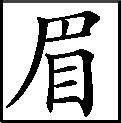
\includegraphics[width=3mm]{../Images/00010}\footnotesize \kaishu 八字为二玉一生文字之纲。}这日不知为何,他二人言语有些不合起来,黛玉又{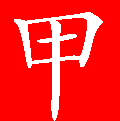
\includegraphics[width=3mm]{../Images/00002}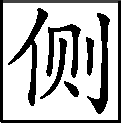
\includegraphics[width=3mm]{../Images/00011}\footnotesize \kaishu ``又''字妙极!补出近日无限垂泪之事矣,此仍淡淡写来,使后文来得不突然。}气的独在房中垂泪,宝玉又{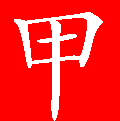
\includegraphics[width=3mm]{../Images/00002}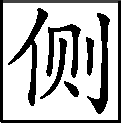
\includegraphics[width=3mm]{../Images/00011}\footnotesize \kaishu ``又''字妙极!凡用二``又''字,如双峰对峙,总补二玉正文。}自悔语言冒撞,前去俯就,那黛玉方渐渐的回转来。

因东边宁府中花园内梅花盛开,{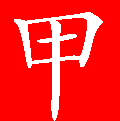
\includegraphics[width=3mm]{../Images/00002}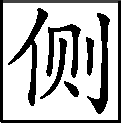
\includegraphics[width=3mm]{../Images/00011}\footnotesize \kaishu 元春消息动矣。}贾珍之妻尤氏乃治酒请贾母、邢夫人、王夫人等赏花。是日,先携了贾蓉之妻二人来面请。贾母等于早饭后过来,就在会芳园{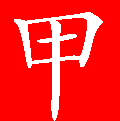
\includegraphics[width=3mm]{../Images/00002}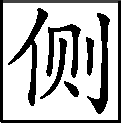
\includegraphics[width=3mm]{../Images/00011}\footnotesize \kaishu 随笔带出,妙!字义可思。}游玩。先茶后酒,不过皆是宁荣二府女眷家宴小集,并无别样新文趣事可记。{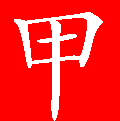
\includegraphics[width=3mm]{../Images/00002}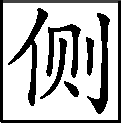
\includegraphics[width=3mm]{../Images/00011}\footnotesize \kaishu 这是第一家宴,偏如此草草写。此如晋人倒食甘蔗,渐入佳境一样。}

一时宝玉倦怠,欲睡中觉,贾母命人好生哄着,歇息一回再来。贾蓉之妻秦氏便忙笑回道:``我们这里有给宝叔收拾下的屋子,老祖宗放心,只管交与我就是了。''又向宝玉的奶娘丫鬟等道:``嬷嬷姐姐们,请宝叔随我这里来。''贾母素知秦氏是个极妥当的人,生得袅娜纤巧,行事又温柔和平,乃重孙媳中第一个得意之人,{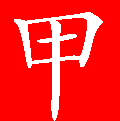
\includegraphics[width=3mm]{../Images/00002}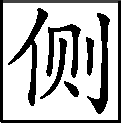
\includegraphics[width=3mm]{../Images/00011}\footnotesize \kaishu 借贾母心中定评,又夹写出秦氏来。}见他去安置宝玉,自是安稳的。

当下秦氏引了一簇人来至上房内间。宝玉抬头看见一幅画贴在上面,画的人物固好,其故事乃是《燃藜图》,也不看系何人所画,心中便有些不快。又有一幅对联,写的是:

世事洞明皆学问,人情练达即文章。{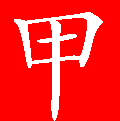
\includegraphics[width=3mm]{../Images/00002}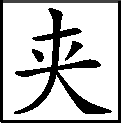
\includegraphics[width=3mm]{../Images/00012}\footnotesize \kaishu 看此联极俗,用于此则极妙。盖作者正为古今王孙公子,劈头先下金针。 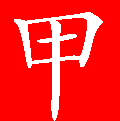
\includegraphics[width=3mm]{../Images/00002}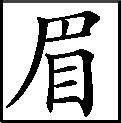
\includegraphics[width=3mm]{../Images/00010}\footnotesize \kaishu 如此画、联,焉能入梦?}

既看了这两句,纵然室宇精美,铺陈华丽,亦断断不肯在这里了,忙说:``快出去!快出去!''秦氏听了笑道:``这里还不好,可往那里去呢?不然往我屋里去吧。''宝玉点头微笑。有一个嬷嬷说道:``那里有个叔叔往侄儿的房里睡觉的礼?''秦氏笑道:``嗳哟哟!不怕他恼。他能多大了,就忌讳这些个!上月你没看见我那个兄弟来了,{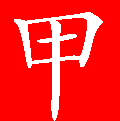
\includegraphics[width=3mm]{../Images/00002}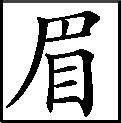
\includegraphics[width=3mm]{../Images/00010}\footnotesize \kaishu 伏下秦钟,妙!}虽然和宝叔同年,两个人若站在一处,只怕那一个还高些呢。''{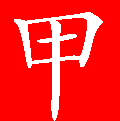
\includegraphics[width=3mm]{../Images/00002}\includegraphics[width=3mm]{../Images/00011}\footnotesize \kaishu 又伏下一人,随笔便出,得隙便入,精细之极。}宝玉道:``我怎么没见过?你带他来我瞧瞧。''{\includegraphics[width=3mm]{../Images/00002}\includegraphics[width=3mm]{../Images/00011}\footnotesize \kaishu 侯门少年纨绔活跳下来。}众人笑道:``隔着二三十里,那里带去?见的日子有呢。''说着,大家来至秦氏房中。刚至房门,便有一股细细的甜香{\includegraphics[width=3mm]{../Images/00002}\includegraphics[width=3mm]{../Images/00011}\footnotesize \kaishu 此香名``引梦香''。}袭了人来。宝玉便愈觉得眼饧骨软,{\includegraphics[width=3mm]{../Images/00002}\includegraphics[width=3mm]{../Images/00011}\footnotesize \kaishu 刻骨吸髓之情景,如何想得来,又如何写得出?}连说:``好香!''{\includegraphics[width=3mm]{../Images/00009}\includegraphics[width=3mm]{../Images/00012}\footnotesize \kaishu 进房如梦境。}入房向壁上看时,有唐伯虎画的《海棠春睡图》,{\includegraphics[width=3mm]{../Images/00002}\includegraphics[width=3mm]{../Images/00011}\footnotesize \kaishu 妙图。}两边有宋学士秦太虚写的一副对联,其联云:

嫩寒锁梦因春冷,{\includegraphics[width=3mm]{../Images/00002}\includegraphics[width=3mm]{../Images/00012}\footnotesize \kaishu 艳极,淫极!}芳气笼人是酒香。{\includegraphics[width=3mm]{../Images/00002}\includegraphics[width=3mm]{../Images/00012}\footnotesize \kaishu 已入梦境矣。}

案上设着武则天当日镜室中设的宝镜,{\includegraphics[width=3mm]{../Images/00002}\includegraphics[width=3mm]{../Images/00011}\footnotesize \kaishu 设譬调侃耳,若真以为然,则又被作者瞒过。}一边摆着飞燕立着舞过的金盘,盘内盛着安禄山掷过伤了太真乳的木瓜。上面设着寿{{(昌)}}{[}阳{]}公主于含章殿下卧的榻,悬的是同昌公主制的联珠帐。宝玉含笑连说:``这里好!''{\includegraphics[width=3mm]{../Images/00009}\includegraphics[width=3mm]{../Images/00012}\footnotesize \kaishu 摆设就合着他的意。}秦氏笑道:``我这屋子,大约神仙也可以住得了。''说着,亲自展开了西子浣过的纱衾,移了红娘抱过的鸳枕。{\includegraphics[width=3mm]{../Images/00002}\includegraphics[width=3mm]{../Images/00011}\footnotesize \kaishu 一路设譬之文,迥非《石头记》大笔所屑,别有他属,余所不知。}于是众奶母伏侍宝玉卧好,款款散去,只留下袭人、{\includegraphics[width=3mm]{../Images/00002}\includegraphics[width=3mm]{../Images/00011}\footnotesize \kaishu 一个再见。}媚人、{\includegraphics[width=3mm]{../Images/00002}\includegraphics[width=3mm]{../Images/00011}\footnotesize \kaishu 二新出。}晴雯、{\includegraphics[width=3mm]{../Images/00002}\includegraphics[width=3mm]{../Images/00011}\footnotesize \kaishu 三新出,名妙而文。}麝月{\includegraphics[width=3mm]{../Images/00002}\includegraphics[width=3mm]{../Images/00011}\footnotesize \kaishu 四新出,尤妙。◇看此四婢之名,则知历来小说难与并肩。}四个丫鬟为伴。{\includegraphics[width=3mm]{../Images/00002}\includegraphics[width=3mm]{../Images/00010}\footnotesize \kaishu 文至此不知从何处想来。}秦氏便分咐小丫鬟们,好生在廊檐下看着猫儿狗儿打架。{\includegraphics[width=3mm]{../Images/00002}\includegraphics[width=3mm]{../Images/00011}\footnotesize \kaishu 细极。}

那宝玉刚合上眼,便惚惚睡去,犹似秦氏在前,遂悠悠荡荡,随了秦氏,至一所在。{\includegraphics[width=3mm]{../Images/00002}\includegraphics[width=3mm]{../Images/00011}\footnotesize \kaishu 此梦文情固佳,然必用秦氏引梦,又用秦氏出梦,竟不知立意何属?◇惟批书人知之。}但见朱栏白石,绿树清溪,真是人迹希逢,飞尘不到。{\includegraphics[width=3mm]{../Images/00002}\includegraphics[width=3mm]{../Images/00011}\footnotesize \kaishu 一篇《蓬莱赋》。}宝玉在梦中欢喜,想道:``这个去处有趣!我就在这里过一生,纵然失了家也愿意,强如天天被父母、师傅打去。''{{\includegraphics[width=3mm]{../Images/00002}\includegraphics[width=3mm]{../Images/00011}\footnotesize \kaishu {(一句)}{[}百{]}忙里点出小儿心性。}}正胡思之间,忽听山后有人作歌曰:

春梦随云散,{\includegraphics[width=3mm]{../Images/00002}\includegraphics[width=3mm]{../Images/00012}\footnotesize \kaishu 开口拿``春''字,最紧要!}飞花逐水流。{\includegraphics[width=3mm]{../Images/00002}\includegraphics[width=3mm]{../Images/00012}\footnotesize \kaishu 二句比也。}

寄言众儿女,何必觅闲愁。{\includegraphics[width=3mm]{../Images/00002}\includegraphics[width=3mm]{../Images/00012}\footnotesize \kaishu 将通部人一喝。}

宝玉听了,是女子的声音。{\includegraphics[width=3mm]{../Images/00002}\includegraphics[width=3mm]{../Images/00011}\footnotesize \kaishu 写出终日与女儿厮混最熟。}歌声未息,早见那边走出一个人来,蹁跹袅娜,端的与人不同。有赋为证:

方离柳坞,乍出花房。但行处,鸟惊庭树;将到时,影度回廊。仙袂乍飘兮,闻麝兰之馥郁;荷衣欲动兮,听环佩之铿锵。靥笑春桃兮,云堆翠髻;唇绽樱颗兮,榴齿含香。纤腰之楚楚兮,回风舞雪;珠翠之辉辉兮,满额鹅黄。出没花间兮,宜嗔宜喜;徘徊池上兮,若飞若扬。蛾眉颦笑兮,将言而未语;莲步乍移兮,欲止而欲行。羡彼之良质兮,冰清玉润;慕彼之华服兮,熌灼文章;爱彼之貌容兮,香培玉琢;美彼之态度兮,凤翥龙翔。其素若何?春梅绽雪。其洁若何?秋菊披霜。其静若何?松生空谷。其艳若何?霞映澄塘。其文若何?龙游曲沼。其神若何?月射寒江。应惭西子,实愧王嫱。吁!奇矣哉,生于孰地,来自何方?信矣乎,瑶池不二,紫府无双。果何人哉?如斯之美也!{\includegraphics[width=3mm]{../Images/00002}\includegraphics[width=3mm]{../Images/00010}\footnotesize \kaishu 按此书凡例,本无赞赋闲文,前有宝玉二词,今复见此一赋,何也?盖此二人乃通部大纲,不得不用此套。前词却是作者别有深意,故见其妙。此赋则不见长,然亦不可无者也。}

宝玉见是一个仙姑,喜的忙上来作揖,笑问道:``神仙姐姐,{\includegraphics[width=3mm]{../Images/00002}\includegraphics[width=3mm]{../Images/00011}\footnotesize \kaishu 千古未闻之奇称,写来竟成千古未闻之奇语。故是千古未有之奇文。}不知从那里来,如今要往那里去?我也不知这里是何处,望乞携带携带。''那仙姑笑道:``吾居离恨天之上,灌愁海之中,乃放春山遣香洞太虚幻境警幻仙姑是也。{\includegraphics[width=3mm]{../Images/00002}\includegraphics[width=3mm]{../Images/00011}\footnotesize \kaishu 与首回中甄士隐梦境一照。}司人间之风情月债,掌尘世之女怨男痴。因近来风流冤孽,{\includegraphics[width=3mm]{../Images/00002}\includegraphics[width=3mm]{../Images/00011}\footnotesize \kaishu 四字可畏。}缠绵于此处,是以前来访察机会,布散相思。今忽与尔相逢,亦非偶然。此离吾境不远,别无他物,仅有自采仙茗一盏,亲酿美酒一瓮,素练魔舞歌姬数人,新填《红楼梦》{\includegraphics[width=3mm]{../Images/00002}\includegraphics[width=3mm]{../Images/00011}\footnotesize \kaishu 点题。盖作者自云所历不过红楼一梦耳。}仙曲十二支,试随吾一游否?''宝玉听了,喜跃非常,便忘了秦氏在何处,{\includegraphics[width=3mm]{../Images/00002}\includegraphics[width=3mm]{../Images/00011}\footnotesize \kaishu 细极。}竟随了仙姑,至一所在,{\includegraphics[width=3mm]{../Images/00009}\includegraphics[width=3mm]{../Images/00012}\footnotesize \kaishu 士隐曾见此匾对,而僧道不能领入,留此回警幻邀宝玉后文。}有石牌横建,上书``太虚幻境''四个大字,两边一副对联,乃是:

假作真时真亦假,无为有处有还无。{{{\includegraphics[width=3mm]{../Images/00002}\includegraphics[width=3mm]{../Images/00012}\footnotesize \kaishu 正恐观者忘却首回,故特将甄士隐梦景重一}滃{染。}}}

转过牌坊,便是一座宫门,也横书四个大字,道是``孽海情天''。又有一副对联,大书云:

厚地高天,堪叹古今情不尽;

痴男怨女,可怜风月债难偿。

宝玉看了,{{\includegraphics[width=3mm]{../Images/00002}\includegraphics[width=3mm]{../Images/00010}\footnotesize \kaishu 菩萨天尊皆因僧道而有,以点俗人,独不许幻造太虚幻境以警情者乎?观者恶其荒唐,余则喜其新鲜。◇有修庙造塔祈福者,余今意欲起太虚幻境,{(以)}{[}似{]}较修七十二司更有功德。}}心下自思道:``原来如此。但不知何为`古今之情',又何为`风月之债'?从今倒要领略领略。''宝玉只顾如此一想,不料早把些邪魔招入膏肓了。{\includegraphics[width=3mm]{../Images/00002}\includegraphics[width=3mm]{../Images/00011}\footnotesize \kaishu 奇极,妙文!}当下随了仙姑进入二层门内,只见两边配殿,皆有匾额、对联,一时看不尽许多,惟见有几处写的是:``痴情司''、``结怨司''、``朝啼司''、``夜哭司''、``春感司''、``秋悲司''。{\includegraphics[width=3mm]{../Images/00002}\includegraphics[width=3mm]{../Images/00011}\footnotesize \kaishu 虚陪六个。}看了,因向仙姑道:``敢烦仙姑引我到那各司中游玩游玩,不知可使得?''仙姑道:``此各司中皆贮的是普天之下所有的女子过去未来的簿册。尔凡眼尘躯,未便先知的。''宝玉听了,那里肯依,复央之再四。仙姑无奈,说:``也罢,就在此司内略随喜随喜罢了。''宝玉喜不自胜,抬头看这司的匾上,乃是``薄命司''{\includegraphics[width=3mm]{../Images/00002}\includegraphics[width=3mm]{../Images/00011}\footnotesize \kaishu 正文。}三字,两边对联写道是:

春恨秋悲皆自惹,花容月貌为谁妍?

宝玉看了,便知{\includegraphics[width=3mm]{../Images/00002}\includegraphics[width=3mm]{../Images/00011}\footnotesize \kaishu ``便知''二字是字法,最为紧要之至。}感叹。

进入门来,只见有十数个大厨,皆用封条封着。看那封条上,皆是各省地名。宝玉一心只拣自己的家乡封条看,遂无心看别省的了。只见那边厨上封条上大书七字云:``金陵十二钗正册''。{\includegraphics[width=3mm]{../Images/00002}\includegraphics[width=3mm]{../Images/00011}\footnotesize \kaishu 正文,点题。}宝玉因问:``何为`金陵十二钗正册'?''警幻道:``即贵省中十二冠首女子之册,故为`正册'。''宝玉道:``常听{\includegraphics[width=3mm]{../Images/00002}\includegraphics[width=3mm]{../Images/00011}\footnotesize \kaishu ``常听''二字,神理极妙。}人说,金陵极大,怎么只十二个女子?如今单我们家里,上上下下,就有几百女孩儿呢。''{\includegraphics[width=3mm]{../Images/00002}\includegraphics[width=3mm]{../Images/00011}\footnotesize \kaishu 贵公子口声。}警幻冷笑道:``贵省女子固多,不过择其紧要者录之。下边二厨则又次之。馀者庸常之辈,则无册可录矣。''宝玉听说,再看下首二厨上,果然一个写着``金陵十二钗副册'',又一个写着``金陵十二钗又副册''。宝玉便伸手先将``又副册''厨门开了,拿出一本册来,揭开一看,只见这首页上画着一幅画,又非人物,亦非山水,不过是水墨滃染的满纸乌云浊雾而已。后有几行字迹,写道是:

霁月难逢,彩云易散。

心比天高,身为下贱。

风流灵巧招人怨。

寿夭多因毁谤生,多情公子空牵念。{\includegraphics[width=3mm]{../Images/00002}\includegraphics[width=3mm]{../Images/00012}\footnotesize \kaishu 恰极之至!``病补雀金裘''回中与此合看。}

宝玉看了,又见后面画着一簇鲜花,一床破席。也有几句言词,写道是:

枉自温柔和顺,空云似桂如兰。

堪羡优伶有福,谁知公子无缘。{\includegraphics[width=3mm]{../Images/00002}\includegraphics[width=3mm]{../Images/00012}\footnotesize \kaishu 骂死宝玉,却是自悔。}

宝玉看了不解。遂掷下这个,又去开了``副册''厨门,拿起一本册来,揭开看时,只见画着一株桂花,下面有一池沼,其中水涸泥干,莲枯藕败。后面书云:

根并荷花一茎香,{\includegraphics[width=3mm]{../Images/00002}\includegraphics[width=3mm]{../Images/00012}\footnotesize \kaishu 却是咏菱妙句。}平生遭际实堪伤。

自从两地生孤木,{\includegraphics[width=3mm]{../Images/00002}\includegraphics[width=3mm]{../Images/00012}\footnotesize \kaishu 拆字法。}致使香魂返故乡。

宝玉看了仍不解。便又掷下,再去取``正册''看。只见头一页上便画着两株枯木,木上悬着一围玉带;又有一堆雪,雪下一股金簪。也有四句言词,道是:

可叹停机德,{{\includegraphics[width=3mm]{../Images/00002}\includegraphics[width=3mm]{../Images/00012}\footnotesize \kaishu 此句薛。 }\includegraphics[width=3mm]{../Images/00005}\includegraphics[width=3mm]{../Images/00012}\footnotesize \kaishu 乐羊子妻事。}堪怜咏絮才,{\includegraphics[width=3mm]{../Images/00002}\includegraphics[width=3mm]{../Images/00012}\footnotesize \kaishu 此句林。}

玉带林中挂,金簪雪里埋。{\includegraphics[width=3mm]{../Images/00002}\includegraphics[width=3mm]{../Images/00012}\footnotesize \kaishu 寓意深远,皆生非其地之意。}

宝玉看了仍不解。{\includegraphics[width=3mm]{../Images/00002}\includegraphics[width=3mm]{../Images/00010}\footnotesize \kaishu 世之好事者争传《推背图》之说,想前人断不肯煽惑愚迷,即有此说,亦非常人供谈之物。此回悉借其法,为儿女子数运之机。无可以供茶酒之物,亦无干涉政事,真奇想奇笔。}待要问时,情知他必不肯泄漏,待要丢下,又不舍。遂又往后看时,只见画着一张弓,弓上挂一香橼。也有一首歌词云:

二十年来辨是非,榴花开处照宫闱。

三春争及初春景,{\includegraphics[width=3mm]{../Images/00002}\includegraphics[width=3mm]{../Images/00012}\footnotesize \kaishu 显极。}虎兔\href{../Text/part0009_split_000.html\#lnkback_2_a}{\textsuperscript{②}}相逢大梦归。

后面又画着两人放风筝,一片大海,一只大船,船中有一女子掩面泣涕之状。也有四句写云:

才自精明志自高,生于末世运偏消。{\includegraphics[width=3mm]{../Images/00002}\includegraphics[width=3mm]{../Images/00012}\footnotesize \kaishu 感叹句,自寓。}

清明涕送江边望,千里东风一梦遥。{\includegraphics[width=3mm]{../Images/00002}\includegraphics[width=3mm]{../Images/00012}\footnotesize \kaishu 好句!}

后面又画几缕飞云,一湾逝水。其词曰:

富贵又何为?襁褓之间父母违。

展眼吊斜晖,湘江水逝楚云飞。

后面又画着一块美玉,落在泥垢之中。其断语云:

欲洁何曾洁,云空未必空。

可怜金玉质,终陷淖泥中。

后面忽画一恶狼,追扑一美女,欲啖之意。其书云:

子系中山狼,得志便猖狂。{\includegraphics[width=3mm]{../Images/00002}\includegraphics[width=3mm]{../Images/00012}\footnotesize \kaishu 好句!}

金闺花柳质,一载赴黄粱。

后面便是一所古庙,里面有一美人在内看经独坐。其判云:

勘破三春景不长,缁衣顿改昔年妆。

可怜绣户侯门女,独卧青灯古佛旁。{\includegraphics[width=3mm]{../Images/00002}\includegraphics[width=3mm]{../Images/00012}\footnotesize \kaishu 好句!}

后面便是一片冰山,上有一只雌凤。其判曰:

凡鸟偏从末世来,都知爱慕此生才。

一从二令三人木,{\includegraphics[width=3mm]{../Images/00002}\includegraphics[width=3mm]{../Images/00012}\footnotesize \kaishu 拆字法。}哭向金陵事更哀。

后面又有一座荒村野店,有一美人在那里纺绩。其判云:

势败休云贵,家亡莫论亲。{\includegraphics[width=3mm]{../Images/00002}\includegraphics[width=3mm]{../Images/00012}\footnotesize \kaishu 非经历过者,此二句则云纸上谈兵。过来人那得不哭!}

偶因济刘氏,巧得遇恩人。

诗后又画一盆茂兰,旁有一位凤冠霞帔的美人。也有判云:

桃李春风结子完,到头谁似一盆兰。

如冰水好空相妒,枉与他人作笑谈。{\includegraphics[width=3mm]{../Images/00002}\includegraphics[width=3mm]{../Images/00012}\footnotesize \kaishu 真心实语。}

后面又画着高楼大厦,有一美人悬梁自缢。其判云:

情天情海幻情身,情既相逢必主淫。

漫言不肖皆荣出,造衅开端实在宁。

宝玉还欲看时,那仙姑知他天分高明,性情颖慧,{\includegraphics[width=3mm]{../Images/00002}\includegraphics[width=3mm]{../Images/00010}\footnotesize \kaishu 通部中笔笔贬宝玉,人人嘲宝玉,语语谤宝玉,今却于警幻意中忽写出此八字来,真是意外之想。此法亦别书中所无。}恐把仙机泄漏,遂掩了卷册,笑向宝玉道:``且随我去游玩奇景,{\includegraphics[width=3mm]{../Images/00002}\includegraphics[width=3mm]{../Images/00011}\footnotesize \kaishu 是哄小儿语,细甚。}何必在此打这闷葫芦!''{\includegraphics[width=3mm]{../Images/00002}\includegraphics[width=3mm]{../Images/00011}\footnotesize \kaishu 为前文``葫芦庙''一点。}

宝玉恍恍惚惚,不觉弃了卷册,{\includegraphics[width=3mm]{../Images/00002}\includegraphics[width=3mm]{../Images/00011}\footnotesize \kaishu 是梦中景况,细极。}又随了警幻来至后面。但见珠帘绣幕,画栋雕檐,说不尽那光摇朱户金铺地,雪照琼窗玉作宫。更见仙花馥郁,异草芬芳,真好个所在。{\includegraphics[width=3mm]{../Images/00002}\includegraphics[width=3mm]{../Images/00011}\footnotesize \kaishu 已为省亲别墅画下图式矣。}又听警幻笑道:``你们快出来迎接贵客!''一语未了,只见房中又走出几个仙子来,皆是荷袂蹁跹,羽衣飘舞,姣若春花,媚如秋月。一见了宝玉,都怨谤警幻道:``我们不知系何`贵客',忙的接了出来!姐姐曾说今日今时必有绛珠妹子{\includegraphics[width=3mm]{../Images/00002}\includegraphics[width=3mm]{../Images/00011}\footnotesize \kaishu 绛珠为谁氏?请观者细思首回。}的生魂前来游玩,故我等久待。何故反引这浊物来污染这清净女儿之境?''{\includegraphics[width=3mm]{../Images/00002}\includegraphics[width=3mm]{../Images/00010}\footnotesize \kaishu 奇笔摅奇文。作书者视女儿珍贵之至,不知今时女儿可知?余为作者痴心一哭,又为近之自弃自败之女儿一恨。}宝玉听如此说,便唬得欲退不能退,{{\includegraphics[width=3mm]{../Images/00002}\includegraphics[width=3mm]{../Images/00011}\footnotesize \kaishu 贵公子不怒而反退,却是宝玉天分中一段情痴。 }\includegraphics[width=3mm]{../Images/00005}\includegraphics[width=3mm]{../Images/00012}\footnotesize \kaishu 贵公子岂容人如此厌弃,反不怒而反欲退,实实写尽宝玉天分中一段情痴来。若是薛阿呆至此,闻是语,则警幻之辈共成齑粉矣。一笑。}果觉自形污秽不堪。警幻忙携住宝玉的手,{\includegraphics[width=3mm]{../Images/00002}\includegraphics[width=3mm]{../Images/00011}\footnotesize \kaishu 妙!警幻自是个多情种子。}向众姊妹道:``你等不知原委:今日原欲往荣府去接绛珠,适从宁府所过,偶遇宁荣二公之灵,嘱吾云:`吾家自国朝定鼎以来,功名奕世,富贵传流,虽历百年,奈运终数尽,不可挽回者。故近之子孙虽多,竟无一可以继业。{\includegraphics[width=3mm]{../Images/00002}\includegraphics[width=3mm]{../Images/00011}\footnotesize \kaishu 这是作者真正一把眼泪。}其中惟嫡孙宝玉一人,禀性乖张,生情怪谲,虽聪明灵慧,略可望成,无奈吾家运数合终,恐无人规引入正。幸仙姑偶来,万望先以情欲声色等事警其痴顽,{\includegraphics[width=3mm]{../Images/00002}\includegraphics[width=3mm]{../Images/00011}\footnotesize \kaishu 二公真无可奈何,开一觉世觉人之路也。}或能使彼跳出迷人圈子,然后入于正路,亦吾兄弟之幸矣。'如此嘱吾,故发慈心,引彼至此。先以彼家上、中、下三等女子之终身册籍,令彼熟玩,尚未觉悟。故引彼再至此处,令其再历饮馔声色之幻,或冀将来一悟,亦未可知也。''{\includegraphics[width=3mm]{../Images/00002}\includegraphics[width=3mm]{../Images/00011}\footnotesize \kaishu 一段叙出宁、荣二公,足见作者深意。}

说毕,携了宝玉入室。但闻一缕幽香,竟不知所焚何物。宝玉遂不禁相问,警幻冷笑道:``此香尘世中既无,尔何能知!此香乃系诸名山胜境内初生异卉之精,合各种宝林珠树之油所制,名为`群芳髓'。''{\includegraphics[width=3mm]{../Images/00002}\includegraphics[width=3mm]{../Images/00011}\footnotesize \kaishu 好香!}宝玉听了,自是羡慕。已而大家入座,小鬟捧上茶来。宝玉自觉清香味异,纯美非常,因又问何名。警幻道:``此茶出在放春山遣香洞,又以仙花灵叶上所带宿露而烹。此茶名曰`千红一窟'。''{\includegraphics[width=3mm]{../Images/00002}\includegraphics[width=3mm]{../Images/00011}\footnotesize \kaishu 隐``哭''字。}宝玉听了,点头称赏。因看房内,瑶琴、宝鼎、古画、新诗,无所不有,更喜窗下亦有唾绒,奁间时渍粉污。{\includegraphics[width=3mm]{../Images/00005}\includegraphics[width=3mm]{../Images/00012}\footnotesize \kaishu 是宝玉心事。}壁上也有一副对联,书云:

幽微灵秀地,{\includegraphics[width=3mm]{../Images/00002}\includegraphics[width=3mm]{../Images/00012}\footnotesize \kaishu 女儿之心,女儿之境。}

无可奈何天。{\includegraphics[width=3mm]{../Images/00002}\includegraphics[width=3mm]{../Images/00012}\footnotesize \kaishu 两句尽矣。撰通部大书不难,最难是此等处,可知皆从无可奈何而有。}

宝玉看毕,无不羡慕。因又请问众仙姑姓名:一名痴梦仙姑,一名钟情大士,一名引愁金女,一名度恨菩提,各各道号不一。少刻,有小鬟来调桌安椅,设摆酒馔。真是:琼浆满泛玻璃盏,玉液浓斟琥珀杯。更不用再说那肴馔之盛。宝玉因闻得此酒清香甘冽,异乎寻常,又不禁相问。警幻道:``此酒乃是百花之蕊,万木之汁,加以麟髓之醅,凤乳之麯酿成,因名为`万艳同杯'。''{\includegraphics[width=3mm]{../Images/00002}\includegraphics[width=3mm]{../Images/00011}\footnotesize \kaishu 与``千红一窟''一对,隐``悲''字。}宝玉称赏不迭。

饮酒间,又有十二个舞女上来,请问演何词曲。警幻道:``就将新制《红楼梦》十二支演上来。''舞女们答应了,便轻敲檀板,款按银筝。听他歌道是:

开辟鸿蒙\ldots{}\ldots{}{\includegraphics[width=3mm]{../Images/00002}\includegraphics[width=3mm]{../Images/00012}\footnotesize \kaishu 故作顿挫摇摆。}

方歌了一句,警幻便说道:``此曲不比尘世中所填传奇之曲,必有生旦净末之别,又有南北九宫之限。此或咏叹一人,或感怀一事,偶成一曲,即可谱入管弦。若非个中人,{\includegraphics[width=3mm]{../Images/00002}\includegraphics[width=3mm]{../Images/00011}\footnotesize \kaishu 三字要紧。不知谁是个中人。宝玉即个中人乎?然则石头亦个中人乎?作者亦系个中人乎?观者亦个中人乎?}不知其中之妙。料尔亦未必深明此调,若不先阅其稿,后听其歌,翻成嚼蜡矣。''{\includegraphics[width=3mm]{../Images/00002}\includegraphics[width=3mm]{../Images/00010}\footnotesize \kaishu 警幻是个极会看戏人。近之大老观戏,必先翻阅角本。目睹其词,耳听彼歌,却从警幻处学来。}说毕,回头命小鬟取了《红楼梦》的原稿来,递与宝玉。宝玉揭开,一面目视其文,一面耳聆其歌曰:{\includegraphics[width=3mm]{../Images/00002}\includegraphics[width=3mm]{../Images/00010}\footnotesize \kaishu 作者能处,惯于自站地步,又惯于陡起波澜,又惯于故为曲折,最是行文秘诀。}

第一支 红楼梦引子

开辟鸿蒙,谁为情种?{\includegraphics[width=3mm]{../Images/00002}\includegraphics[width=3mm]{../Images/00011}\footnotesize \kaishu 非作者为谁?余又曰:``亦非作者,乃石头耳。''}都只为风月情浓。趁着这奈何天、伤怀日、寂寥时,试遣愚{\includegraphics[width=3mm]{../Images/00002}\includegraphics[width=3mm]{../Images/00011}\footnotesize \kaishu ``愚''字自谦得妙!}衷。因此上,演出这怀金悼玉的《红楼梦》。{\includegraphics[width=3mm]{../Images/00002}\includegraphics[width=3mm]{../Images/00012}\footnotesize \kaishu 读此几句,翻厌近之传奇中必用开场副末等套,累赘太甚。 \includegraphics[width=3mm]{../Images/00002}\includegraphics[width=3mm]{../Images/00010}\footnotesize \kaishu ``怀金悼玉'',大有深意。}

第二支 终身误

都道是金玉良姻,俺只念木石前盟。空对着山中高士晶莹雪,终不忘世外仙姝寂寞林。叹人间,美中不足今方信。纵然是齐眉举案,到底意难平。{\includegraphics[width=3mm]{../Images/00002}\includegraphics[width=3mm]{../Images/00010}\footnotesize \kaishu 语句泼撒,不负自创北曲。}

第三支 枉凝眉

一个是阆苑仙葩,一个是美玉无瑕。若说没奇缘,今生偏又遇着他;若说有奇缘,如何心事终虚化?一个枉自嗟呀,一个空劳牵挂。一个是水中月,一个是镜中花。想眼中能有多少泪珠儿,怎经得秋流到冬尽,春流到夏!

宝玉听了此曲,散漫无稽,不见得好处,{\includegraphics[width=3mm]{../Images/00002}\includegraphics[width=3mm]{../Images/00011}\footnotesize \kaishu 自批驳,妙极!}但其声韵凄惋,竟能销魂醉魄。因此也不察其原委,问其来历,就暂以此释闷而已。{\includegraphics[width=3mm]{../Images/00002}\includegraphics[width=3mm]{../Images/00010}\footnotesize \kaishu 妙!设言世人亦应如此法看此《红楼梦》一书,更不必追究其隐寓。}因又看下面道:

第四支 恨无常

喜荣华正好,恨无常又到。眼睁睁把万事全抛,荡悠悠把芳魂消耗。望家乡,路远山高。故向爹娘梦里相寻告:儿命已入黄泉,天伦呵,须要退步抽身早!{\includegraphics[width=3mm]{../Images/00002}\includegraphics[width=3mm]{../Images/00012}\footnotesize \kaishu 悲险之至!}

第五支 分骨肉

一帆风雨路三千,把骨肉家园齐来抛闪。恐哭损残年,告爹娘,休把儿悬念。自古穷通皆有定,离合岂无缘?从今分两地,各自保平安。奴去也,莫牵连!{\includegraphics[width=3mm]{../Images/00005}\includegraphics[width=3mm]{../Images/00012}\footnotesize \kaishu 探卿声口如闻。}

第六支 乐中悲

襁褓中,父母叹双亡。{\includegraphics[width=3mm]{../Images/00002}\includegraphics[width=3mm]{../Images/00011}\footnotesize \kaishu 意真辞切,过来人见之不免失声。}纵居那绮罗丛,谁知娇养?幸生来英豪阔大宽宏量,从未将儿女私情略萦心上。好一似霁月光风耀玉堂。{\includegraphics[width=3mm]{../Images/00005}\includegraphics[width=3mm]{../Images/00012}\footnotesize \kaishu 堪与湘卿作照。}厮配得才貌仙郎,博得个地久天长,准折得幼年时坎坷形状。终久是云散高唐,水涸湘江。这是尘寰中消长数应当,何必枉悲伤!{\includegraphics[width=3mm]{../Images/00002}\includegraphics[width=3mm]{../Images/00010}\footnotesize \kaishu 悲壮之极,北曲中不能多得。}

第七支 世难容

气质美如兰,才华阜比仙。{\includegraphics[width=3mm]{../Images/00002}\includegraphics[width=3mm]{../Images/00011}\footnotesize \kaishu 妙卿实当得起。}天生成孤僻人皆罕。你道是啖肉食腥膻,{\includegraphics[width=3mm]{../Images/00002}\includegraphics[width=3mm]{../Images/00011}\footnotesize \kaishu 绝妙!曲文填词中不能多见。}视绮罗俗厌。却不知太高人愈妒,过洁世同嫌。{\includegraphics[width=3mm]{../Images/00002}\includegraphics[width=3mm]{../Images/00012}\footnotesize \kaishu 至语。}可叹这青灯古殿人将老,辜负了红粉朱楼春色阑。到头来,依旧是风尘肮脏违心愿。好一似无瑕白玉遭泥陷,又何须王孙公子叹无缘。

第八支 喜冤家{\includegraphics[width=3mm]{../Images/00005}\includegraphics[width=3mm]{../Images/00012}\footnotesize \kaishu ``冤家''上加一``喜''字,真新真奇!}

中山狼,无情兽,全不念当日根由。一味的骄奢淫荡贪还构。觑着那侯门艳质同蒲柳,作践的公府千金似下流。叹芳魂艳魄,一载荡悠悠。{\includegraphics[width=3mm]{../Images/00002}\includegraphics[width=3mm]{../Images/00012}\footnotesize \kaishu 题只十二钗,却无人不有,无事不备。}

第九支 虚花悟

将那三春看破,桃红柳绿待如何?把这韶华打灭,觅那清淡天和。说什么天上夭桃盛,{\includegraphics[width=3mm]{../Images/00005}\includegraphics[width=3mm]{../Images/00012}\footnotesize \kaishu 此休恰甚。}云中杏蕊多。到头来谁见把秋捱过?则看那白杨村里人呜咽,青枫林下鬼吟哦。更兼着连天衰草遮坟墓。这的是昨贫今富人劳碌,春荣秋谢花折磨。似这般生关死劫谁能躲?闻说道西方宝树唤婆娑,上结着长生果。{\includegraphics[width=3mm]{../Images/00002}\includegraphics[width=3mm]{../Images/00012}\footnotesize \kaishu 末句开句收句。}

第十支 聪明累

机关算尽太聪明,反算了卿卿性命。{{\includegraphics[width=3mm]{../Images/00002}\includegraphics[width=3mm]{../Images/00011}\footnotesize \kaishu 警拔之句。 }\includegraphics[width=3mm]{../Images/00005}\includegraphics[width=3mm]{../Images/00012}\footnotesize \kaishu 喝醒大众,是极。}生前心已碎,死后性空灵。家富人宁,终有个家亡人散各奔腾。{\includegraphics[width=3mm]{../Images/00002}\includegraphics[width=3mm]{../Images/00010}\footnotesize \kaishu 过来人睹此,宁不放声一哭?}枉费了意悬悬半世心,好一似荡悠悠三更梦。忽喇喇似大厦倾,昏惨惨似灯将尽。呀!一场欢喜忽悲辛。叹人世,终难定!{\includegraphics[width=3mm]{../Images/00002}\includegraphics[width=3mm]{../Images/00012}\footnotesize \kaishu 见得到。}

第十一支 留馀庆

留馀庆,留馀庆,忽遇恩人;幸娘亲,幸娘亲,积得阴功。劝人生,济困扶穷,休似俺那爱银钱、忘骨肉的狠舅奸兄!正是乘除加减,上有苍穹。

第十二支 晚韶华

镜里恩情,{\includegraphics[width=3mm]{../Images/00002}\includegraphics[width=3mm]{../Images/00012}\footnotesize \kaishu 起得妙!}更那堪梦里功名!那美韶华去之何迅!再休提绣帐鸳衾。只这带珠冠、披凤袄,也抵不了无常性命。虽说是、人生莫受老来贫,也须要阴骘积儿孙。气昂昂头戴簪缨,气昂昂头戴簪缨,光灿灿胸悬金印;威赫赫爵禄高登,威赫赫爵禄高登,昏惨惨黄泉路近。问古来将相可还存?也只是、虚名儿与后人钦敬。

第十三支 好事终

画梁春尽落香尘。{\includegraphics[width=3mm]{../Images/00002}\includegraphics[width=3mm]{../Images/00011}\footnotesize \kaishu 六朝妙句。}擅风情,秉月貌,便是败家的根本。箕裘颓堕皆从敬\href{../Text/part0009_split_000.html\#lnkback_3_a}{\textsuperscript{③}},{\includegraphics[width=3mm]{../Images/00002}\includegraphics[width=3mm]{../Images/00011}\footnotesize \kaishu 深意,他人不解。}家事消亡首罪宁。宿孽总因情。{\includegraphics[width=3mm]{../Images/00002}\includegraphics[width=3mm]{../Images/00012}\footnotesize \kaishu 是作者具菩萨之心,秉刀斧之笔,撰成此书,一字不可更,一语不可少。}

第十四支{收尾} 飞鸟各投林{\includegraphics[width=3mm]{../Images/00002}\includegraphics[width=3mm]{../Images/00012}\footnotesize \kaishu 收尾愈觉悲惨可畏。}

为官的家业凋零,富贵的金银散尽。{\includegraphics[width=3mm]{../Images/00002}\includegraphics[width=3mm]{../Images/00011}\footnotesize \kaishu 二句先总宁荣。}有恩的死里逃生,无情的分明报应。欠命的命已还,欠泪的泪已尽。冤冤相报岂非轻,分离聚合皆前定。欲知命短问前生,老来富贵也真侥幸。看破的遁入空门,痴迷的枉送了性命。{\includegraphics[width=3mm]{../Images/00002}\includegraphics[width=3mm]{../Images/00011}\footnotesize \kaishu 将通部女子一总。}好一似食尽鸟投林,落了片白茫茫大地真干净!{\includegraphics[width=3mm]{../Images/00002}\includegraphics[width=3mm]{../Images/00012}\footnotesize \kaishu 又照看``葫芦庙''。与``树倒猢狲散''反照。}

歌毕,还要歌副曲。{\includegraphics[width=3mm]{../Images/00002}\includegraphics[width=3mm]{../Images/00011}\footnotesize \kaishu 是极!香菱、晴雯辈岂可无,亦不必再。}警幻见宝玉甚无趣味,{\includegraphics[width=3mm]{../Images/00005}\includegraphics[width=3mm]{../Images/00012}\footnotesize \kaishu 自站地步。}因叹:``痴儿竟尚未悟!''那宝玉忙止歌姬不必再唱,自觉朦胧恍惚,告醉求卧。警幻便命撤去残席,送宝玉至一香闺绣阁之中,其间铺陈之盛,乃素所未见之物。更可骇者,早有一位女子在内,其鲜艳妩媚,有似乎宝钗,风流袅娜,则又如黛玉。{\includegraphics[width=3mm]{../Images/00002}\includegraphics[width=3mm]{../Images/00011}\footnotesize \kaishu 难得双兼,妙极!}正不知何意,忽警幻道:``尘世中多少富贵之家,那些绿窗风月,绣阁烟霞,皆被淫污纨袴与那些流荡女子悉皆玷辱。{\includegraphics[width=3mm]{../Images/00002}\includegraphics[width=3mm]{../Images/00011}\footnotesize \kaishu 真极!}更可恨者,自古来多少轻薄浪子,皆以`好色不淫'为饰,又以`情而不淫'作案,{\includegraphics[width=3mm]{../Images/00005}\includegraphics[width=3mm]{../Images/00012}\footnotesize \kaishu ``色而不淫''四字已滥熟于各小说中,今却特贬其说,批驳出矫饰之非,可谓至切至当,亦可以唤醒众人,勿为前人之矫词所惑也。}此皆饰非掩丑之语也。好色即淫,知情更淫。是以巫山之会,云雨之欢,皆由既悦其色,复恋其情所致也。{\includegraphics[width=3mm]{../Images/00002}\includegraphics[width=3mm]{../Images/00011}\footnotesize \kaishu ``色而不淫'',今翻案,奇甚!}吾所爱汝者,乃天下古今第一淫人也!''{{\includegraphics[width=3mm]{../Images/00002}\includegraphics[width=3mm]{../Images/00011}\footnotesize \kaishu 多大胆量敢作如此之文! }\includegraphics[width=3mm]{../Images/00005}\includegraphics[width=3mm]{../Images/00012}\footnotesize \kaishu 不见下文,使人一惊。多大胆量,敢如此作文。}

宝玉听了,唬的忙答道:``仙姑错了。我因懒于读书,家父母尚每垂训饬,岂敢再冒`淫'字?况且年纪尚小,不知`淫'字为何物。''{\includegraphics[width=3mm]{../Images/00002}\includegraphics[width=3mm]{../Images/00010}\footnotesize \kaishu 绛芸轩中诸事情景由此而生。}警幻道:``非也。淫虽一理,意则有别。如世之好淫者,不过悦容貌,喜歌舞,调笑无厌,云雨无时,恨不能尽天下之美女供我片时之趣兴,{\includegraphics[width=3mm]{../Images/00002}\includegraphics[width=3mm]{../Images/00011}\footnotesize \kaishu 说得恳切,恰当之至!}此皆皮肤滥淫之蠢物耳。如尔则天分中生成一段痴情,吾辈推之为`意淫'。{\includegraphics[width=3mm]{../Images/00002}\includegraphics[width=3mm]{../Images/00011}\footnotesize \kaishu 二字新雅。}`意淫'二字,惟心会而不可口传,可神通而不能语达。{\includegraphics[width=3mm]{../Images/00002}\includegraphics[width=3mm]{../Images/00011}\footnotesize \kaishu 按宝玉一生心性,只不过是``体贴''二字,故曰``意淫''。}汝今独得此二字,在闺阁中,固可为良友,然于世道中未免迂阔怪诡,百口嘲谤,万目睚眦。今既遇令祖宁荣二公剖腹深嘱,吾不忍君独为我闺阁增光,见弃于世道,是以特引前来,醉以灵酒,沁以仙茗,警以妙曲,再将吾妹一人,乳名兼美{\includegraphics[width=3mm]{../Images/00002}\includegraphics[width=3mm]{../Images/00011}\footnotesize \kaishu 妙!盖指薛、林而言也。}字可卿者,许配于汝。今夕良时,即可成姻。不过令汝领略此仙闺幻境之风光尚然如此,何况尘境之情景哉?而今后万万解释,改悟前情,将谨勤有用的工夫,置身于经济之道。\href{../Text/part0009_split_000.html\#lnkback_4_a}{\textsuperscript{④}}''{\includegraphics[width=3mm]{../Images/00005}\includegraphics[width=3mm]{../Images/00012}\footnotesize \kaishu 说出此二句,警幻亦腐矣,然亦不得不然耳。}说毕,便秘授以云雨之事,{\includegraphics[width=3mm]{../Images/00005}\includegraphics[width=3mm]{../Images/00012}\footnotesize \kaishu 这是情之未了一着,不得不说破。}推宝玉入帐。

那宝玉恍恍惚惚,依警幻所嘱之言,未免有阳台、巫峡之会。{\includegraphics[width=3mm]{../Images/00005}\includegraphics[width=3mm]{../Images/00012}\footnotesize \kaishu 如此方免累赘。}数日来,\href{../Text/part0009_split_000.html\#lnkback_5_a}{\textsuperscript{⑤}}柔情缱绻,软语温存,与可卿难解难分。

那日,警幻携宝玉、可卿闲游。至一个所在,但见荆榛遍地,{\includegraphics[width=3mm]{../Images/00005}\includegraphics[width=3mm]{../Images/00012}\footnotesize \kaishu 略露心迹。}狼虎同群。{\includegraphics[width=3mm]{../Images/00005}\includegraphics[width=3mm]{../Images/00012}\footnotesize \kaishu 凶极!试问观者此系何处。}忽尔大河阻路,黑水淌洋,又无桥梁可通。{\includegraphics[width=3mm]{../Images/00002}\includegraphics[width=3mm]{../Images/00011}\footnotesize \kaishu 若有桥梁可通,则世路人情犹不算艰难。}宝玉正自旁徨,只听警幻道:``宝玉休前进,作速回头要紧!''{\includegraphics[width=3mm]{../Images/00002}\includegraphics[width=3mm]{../Images/00011}\footnotesize \kaishu 机锋。}宝玉忙止步问道:``此系何处?''警幻道:``此即迷津也。深有万丈,遥亘千里,中无舟楫可通,{\includegraphics[width=3mm]{../Images/00005}\includegraphics[width=3mm]{../Images/00012}\footnotesize \kaishu 可思。}只有一个木筏,乃木居士掌舵,灰侍者撑篙,{\includegraphics[width=3mm]{../Images/00005}\includegraphics[width=3mm]{../Images/00012}\footnotesize \kaishu 特用``形如槁木,心如死灰''句以消其念,可谓善于读矣。}不受金银之谢,但遇有缘者渡之。尔今偶游至此,如堕落其中,则深负我从前一番以情悟道、守理衷情之言矣。''{\includegraphics[width=3mm]{../Images/00005}\includegraphics[width=3mm]{../Images/00012}\footnotesize \kaishu 看他忽转笔作此语,则知此后皆是自悔。}宝玉方欲回言,只听迷津内水响如雷,竟有一夜叉般怪物窜出,直扑而来\href{../Text/part0009_split_000.html\#lnkback_6_a}{\textsuperscript{⑥}}。吓得宝玉汗下如雨,一面失声喊叫:``可卿救我!可卿救我!''慌得袭人、媚人等上来扶起,拉手说:``宝玉别怕,我们在这里!''{\includegraphics[width=3mm]{../Images/00005}\includegraphics[width=3mm]{../Images/00012}\footnotesize \kaishu 接得无痕迹。历来小说中之梦未见此一醒。}

秦氏在外听见,连忙进来,一面说ㄚ鬟们,好生看着猫儿狗儿打架。{\includegraphics[width=3mm]{../Images/00005}\includegraphics[width=3mm]{../Images/00012}\footnotesize \kaishu 细,又是照应前文。}又闻宝玉口中连叫:``可卿救我'',{\includegraphics[width=3mm]{../Images/00005}\includegraphics[width=3mm]{../Images/00012}\footnotesize \kaishu 奇奇怪怪之文,令人摸透不着。 {\includegraphics[width=3mm]{../Images/00002}\includegraphics[width=3mm]{../Images/00011}\footnotesize \kaishu 云龙作雨,不知何为龙,何为云,何为雨。}}因纳闷道:``我的小名这里没人知道,他如何从梦里叫出来?''正是:

一场幽梦同谁近,千古情人独我痴。\href{../Text/part0009_split_000.html\#lnkback_7_a}{\textsuperscript{⑦}}

{\includegraphics[width=3mm]{../Images/00005}总评:将一部全盘点出几个,以陪衬宝玉。使宝玉从此倍偏倍痴,倍聪明倍潇洒,亦非突如其来。作者真妙心妙口,妙笔妙人。}

{\href{../Text/part0009_split_000.html\#navto_1_a}{①}底本无此回前诗,己本(贴条)、戚本、蒙本、杨本、舒本等有,据补。}

{\href{../Text/part0009_split_000.html\#navto_2_a}{②}``虎兔'',己本、杨本作``虎兕''。}有人据此{认为此句暗示元春死于两派政治势力的恶斗之中。}

{\href{../Text/part0009_split_000.html\#navto_3_a}{③}``从敬'',庚、戚、蒙、舒、甲辰诸本同。惟己本作``荣玉'',杨本作``莹玉''。按前文可卿判词末两句以``荣''、``宁''对举,则此己本之独异文字就值得注意,以``皆荣玉''对``首罪宁'',似较``皆从敬''稍胜。}

{\href{../Text/part0009_split_000.html\#navto_4_a}{④}\href{../Text/part0009_split_000.html\#navto_5_a}{⑤}\href{../Text/part0009_split_000.html\#navto_6_a}{⑥}按:第五回结尾部分,各本与底本间有一些异文,常引起研究者的注意。现据己本择要对照如下(他本个别文字有出入):}

{``将谨勤有用的工夫,置身于经济之道'':``留意于孔孟之间,委身于经济之道''。}

{``未免有阳台、巫峡之会。数日来,'':``未免有儿女之事,难以尽述。至次日,便''。}

{``那日,警幻携宝玉''一段:``因二人携手出去游玩之时,忽至一个所在,但见荆榛遍地,狼虎同群,迎面一道黑溪阻路,并无桥梁可通。正在犹豫之间,忽见警幻从后追来,告道:`快休前进,作速回头要紧!'宝玉忙止步问道:`此系何处?'警幻道:`此即迷津也。\ldots{}\ldots{}尔今偶游至此,设如堕落其中,则深负我从前谆谆警戒之语矣。'话犹未了,只听迷津内水响如雷,竟有许多夜叉海鬼将宝玉拖将下去。''}

{\href{../Text/part0009_split_000.html\#navto_7_a}{⑦}``正是\ldots{}\ldots{}''原无,据庚、戚、蒙、舒等本补。己、杨本联语作:``梦同谁诉离愁恨,千古情人独我知。''}
